\section{Discussion and Conclusion}
Now for a final comparison of all the methods demonstrated in this report, let us solve the Van der Pol problem. The solutions are all computed using an adaptive step size with $abstol = reltol = 10^{-4}$. For solvers that do not have an embedded error estimation, step doubling is used. The result can be seen in in Figure \ref{fig:7_5pp}, \ref{fig:7_5x1} and \ref{fig:7_5x2}.

\\\

All methods solves the problem fairly well. One interesting pattern as seen in Figure \ref{fig:7_5pp}, DOPRI54 likes to cut corners. It gets away with it because it is actually quite precise in the specific points in which it lands, but the linear interpolation between points is quite off. In many applications one would want the numerical solution to the ODE to represent the full behaviour of the system, making the cut-of-corner unfavourable.\\

Comparing ESDIRK23 to the other solvers it performs quite well. Comparing it mainly to DOPRI54 and \textit{ode45} it seen that ESDIRK23 requires more steps on the non-stiff problem for ensuring the specified tolerances. However on the stiff problem, ESDIRK23 uses fewer steps than both DOPRI54 and \textit{ode45} (and even \textit{ode15s}). Clearly, due to it's inherent implicit properties, it is well suited for stiff problems.\\
The Implicit Euler does not get a way with as many fewer steps on the stiff-problem as one might expect when comparing it to the Explicit Euler. Clearly the Classical Runge-Kutta is a strong improvement in number of steps compared to the other two.


\begin{figure}[H]
    \centering
    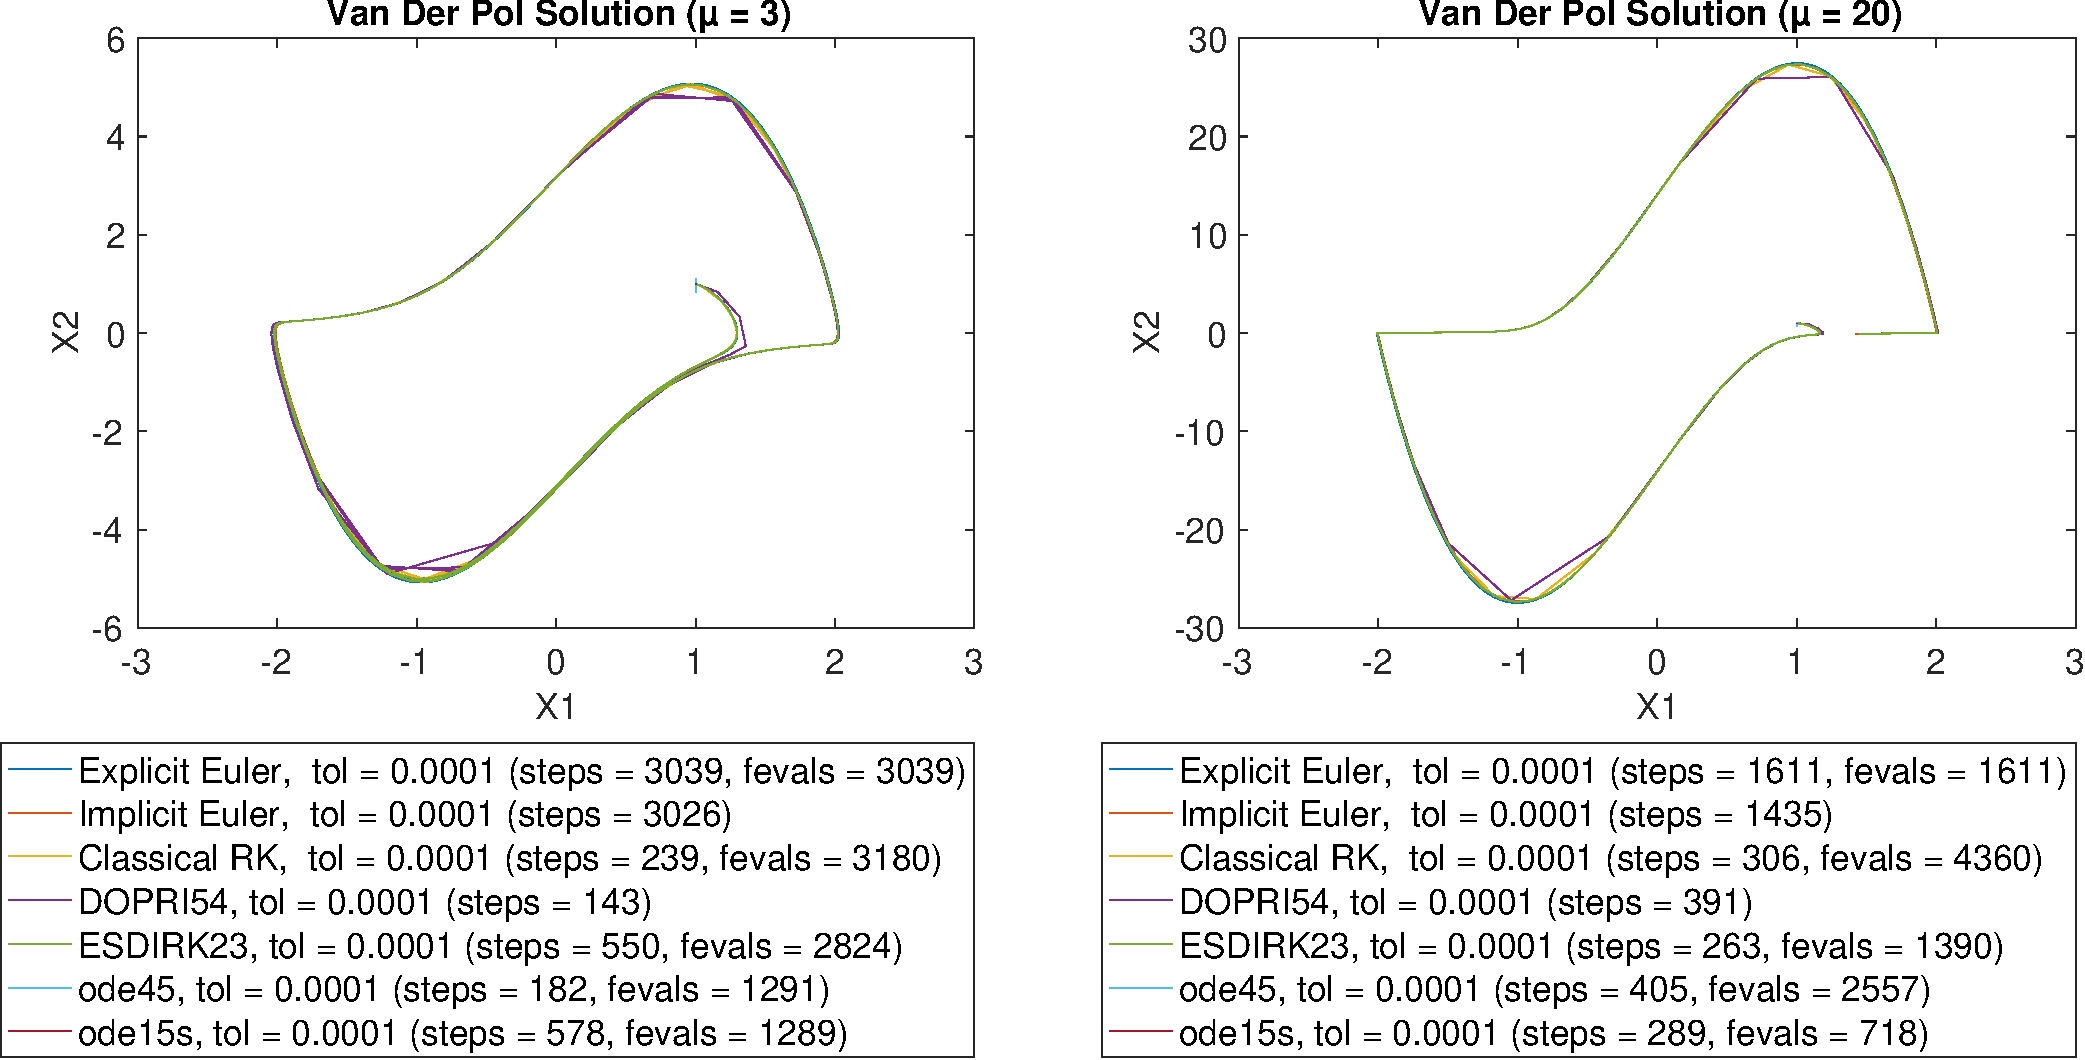
\includegraphics[width=\textwidth]{plots/7_5b.pdf}
    \caption{Phase portraits of the Van der Pol for different solvers.}
    \label{fig:7_5pp}
\end{figure}

\begin{figure}[H]
    \centering
    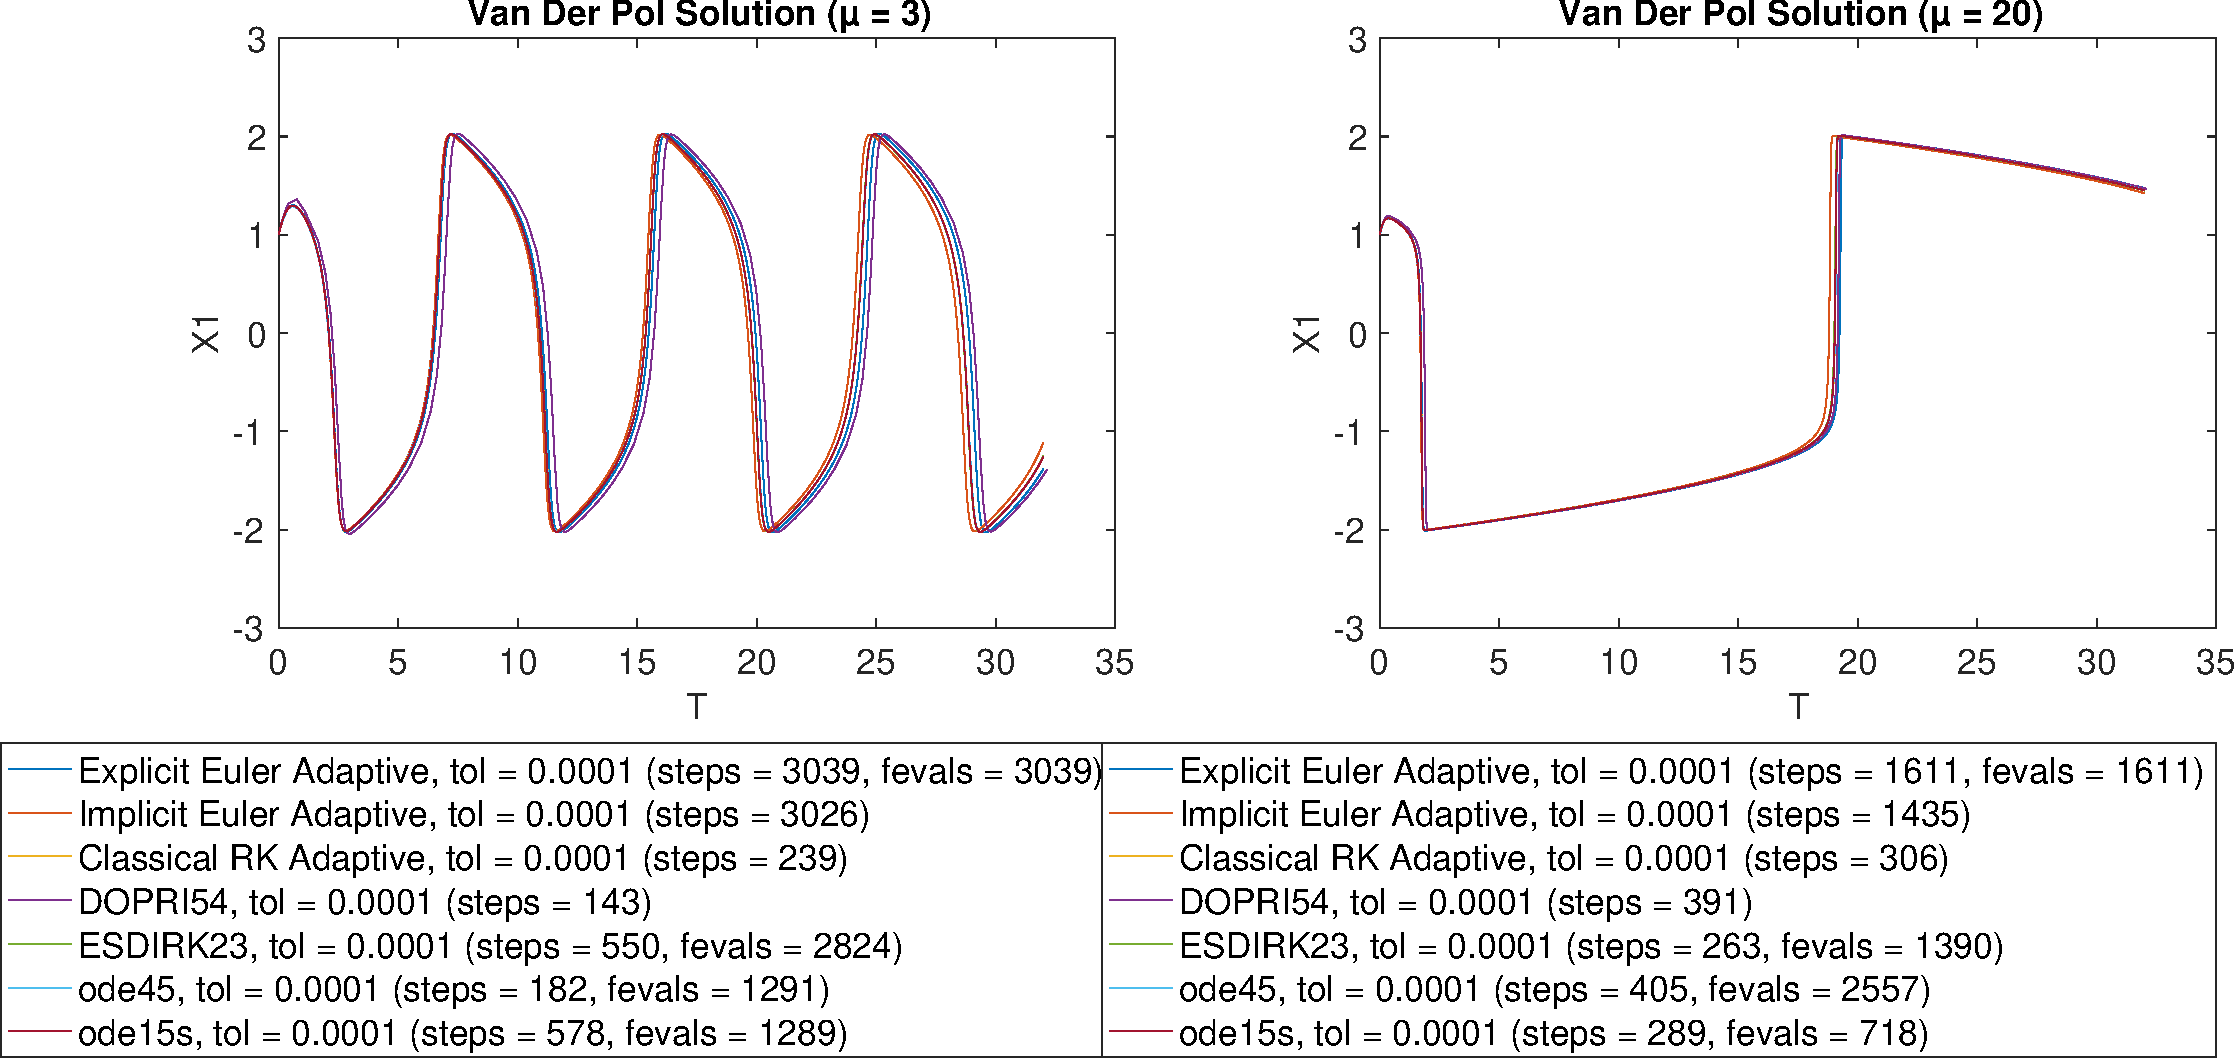
\includegraphics[width=\textwidth]{plots/7_5_X1.pdf}
    \caption{Solution of X1 from the Van der Pol for different solvers.}
    \label{fig:7_5x1}
\end{figure}

\begin{figure}[H]
    \centering
    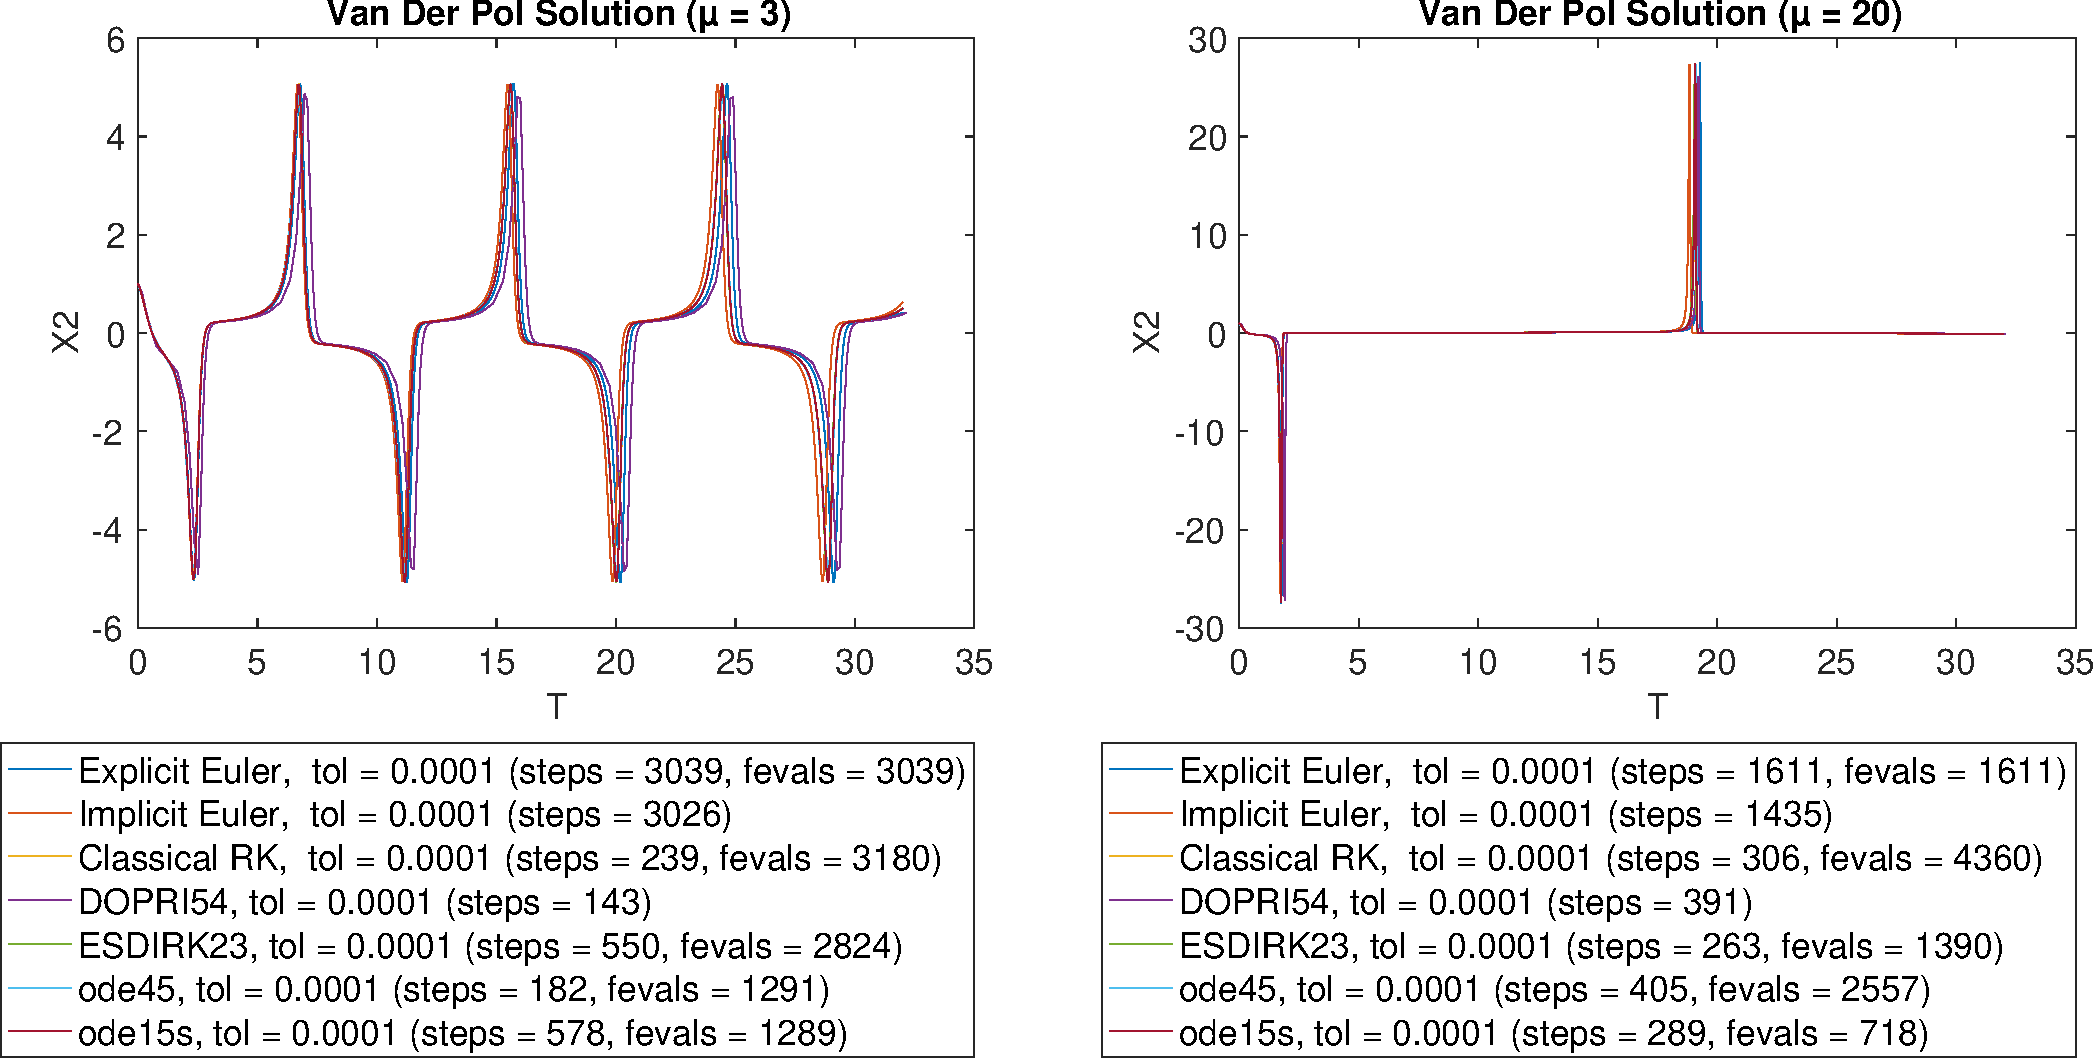
\includegraphics[width=\textwidth]{plots/7_5_X2.pdf}
    \caption{Solution of X1 from the Van der Pol for different solvers.}
    \label{fig:7_5x2}
\end{figure}










% Having just compared all methods on the Van der Pol problem, this report will end with a final comparison on the test equation.

% \begin{equation}
%     \dot{x} = \lambda x(t), \quad x(0) = x_0
% \end{equation}

% For $\lambda = -1$ and $x_0 = 1$. The final comparison is seen in Figure \ref{fig:final}.

% \begin{figure}[H]
%     \centering
%     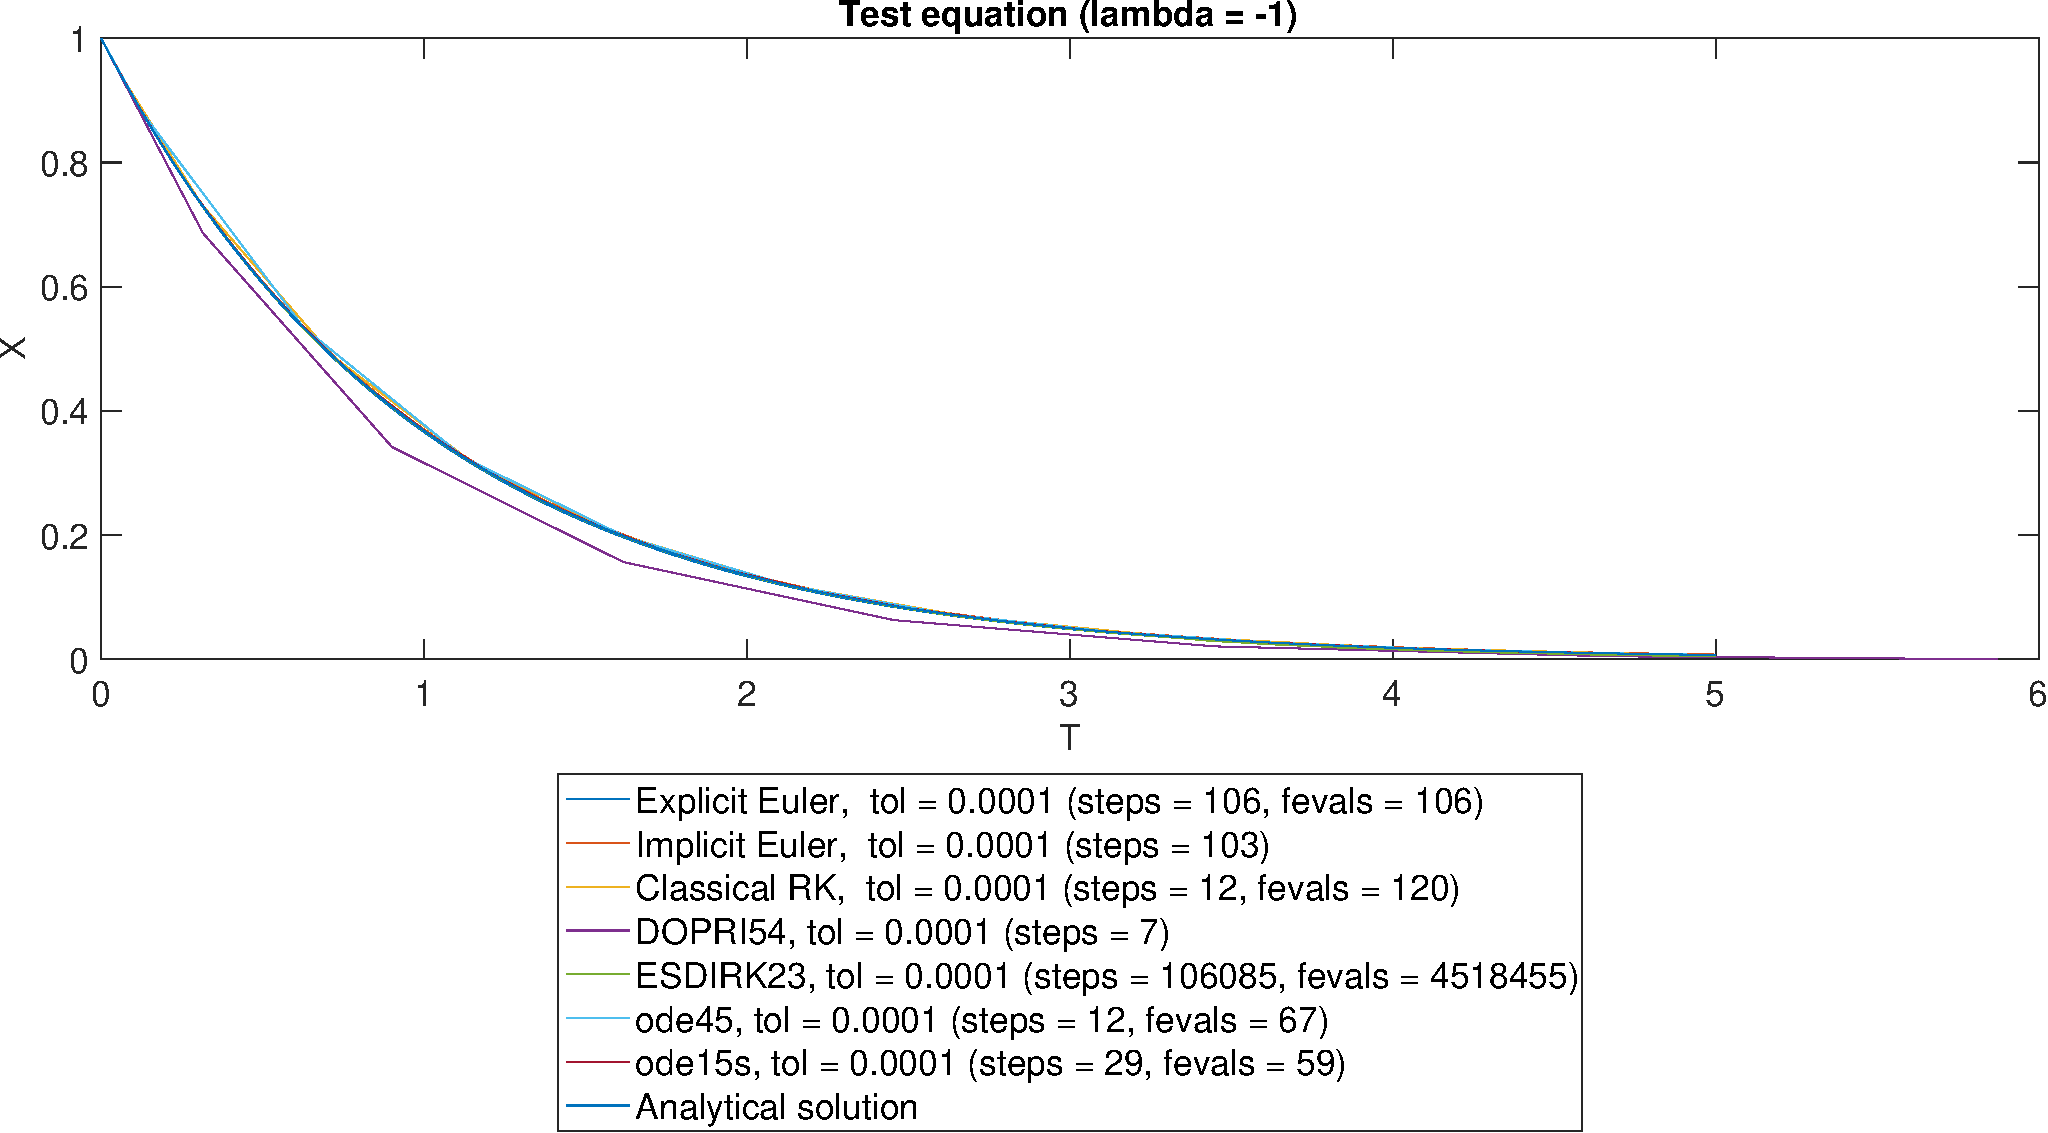
\includegraphics[width=\textwidth]{plots/8a.pdf}
%     \caption{Solution of test equation using various solvers.}
%     \label{fig:final}
% \end{figure}

%Relating to ESDIRK23 steps and function evaluations, clearly something is off with the DAE implementation of the test equation.

\\\

More generally speaking, a variety of numerical ODE solvers has been presented throughout this report. All of them are based on a finite difference discretization of the continuous differential equations. The \textit{Explicit Euler} is the simplest (conceptually and computationally) method which is a good first start since it is fast but inaccurate. Recall though that it is exactly accurate for infinitesimal step size. But for non-infinitesimal step size, the stability region of the method is fairly limited as seen in Section 1.6. \\
If one is interested in a larger stability region the \textit{Implicit Euler} is a good extension. This allows for the method to be run with a higher certainty of the solution converging properly and not blowing up unstably or adhere to take extremely small steps. This is particularly of interest when solving stiff problems. However the Implicit Euler does not come with a higher accuracy (both are 1st order methods) and since it inherently uses Newton's Method, the number of function evaluation can be very high. So the increased stability region might come at a high cost.
\\
A generalisation of both methods are the Runge-Kutta methods which allows for in-between stages in calculating the final forward step $x_{n+1}$. This allows for higher order methods allowing the user to choose an almost arbitrarily accurate method. As we have seen, choosing the coefficients cleverly give rise to classical Runge-Kutta, DOPRI54 and ESDIRK23.
\\
The \textit{Classical Runge-Kutta} performs fairly well. It is an \textit{explicit} 4th order method which has similar cheapness benefits as the Explicit Euler but also the same potential problems with stability. However it does not come with an embedded error estimation for which the step size can be controlled adaptively.\\
\textit{DOPRI54} is a natural extension with an embedded error estimation allowing for adaptively changing the step size. It is purely explicit and has a high accuracy (a order 5 method) which often makes it a good choice of solver for non-stiff problems. This is why MATLAB's \textit{ode45} is an implementation of such. However it does have 7 stages making it more expensive than the classical Runge-Kutta. More importantly, for stiff problems one would typically chose a method with a greater stability.\\
\textit{ESDIRK23} is an example of such a method. Not only is it A-stable, it is also L-stable making it well-suited for stiff problems. This allows for the method to maintain a fairly large step size even in stiff regions of the ODE. 

\\\

In another area, namely the generalisation of ODEs to allow for non-zero stochasticity thereby modelling the world as it is - non-deterministic (atleast from our epistemically limited perspective) - we have seen two solver for stochastic differential equations. Here we have seen that we can use basic ODE solvers for solving the drift term and solving the diffusion term independently using an explicit method.